\documentclass{article}
\usepackage[utf8]{inputenc}
\usepackage[a4paper, total={6in, 8in}]{geometry}

\usepackage{algorithm}
\usepackage{algpseudocode}
\usepackage{amsmath}
\newcommand\ddfrac[2]{\frac{\displaystyle #1}{\displaystyle #2}}
\usepackage{graphicx}
\usepackage[dvipsnames]{xcolor}
\usepackage[colorlinks=true,urlcolor=Blue,linkcolor=Blue,citecolor=Blue]{hyperref}

\title{INFO-H410 Project}
\author{PARDON Mathieu, DIAZ Y SUAREZ Esteban, WAFFLARD Guillaume}
\date{June 2022}

% Content of report:
%   - The content of your project
%   - The theory and AI algorithms underlying it
%   - Some snapshots of your running code.

\begin{document}

\maketitle
\tableofcontents
\clearpage


\section{Introduction}

This report will give a description of the implementation of the artificial intelligence for the turn-based strategy game Othello\copyright. In this game, two players play against each other on an 8×8 square board. The board contains initially 2 pieces of each color (black and white) disposed alternatively in the center of the board. Players take turns placing a piece of their own color on the board (the spaces where pieces can be placed must meet certain constraints) and thus all pieces of the opponent's color that are between two pieces of the player's color are converted into the player's color. The game ends when the board is completely filled with pieces or when neither player has any more moves available. The player with the most pieces of his color on the board wins the game. In order to compare several artificial intelligence methods on this game, we developed a machine learning algorithm and a search algorithm. Machine learning agents have been trained with different hyper-parameters and all types of agents have been tested against each other.

\section{Machine learning agent}

\subsection{Structure of the network}

\subsubsection{Game state encoding}

For the neural networks operations, a game state is represented with one-hot encoding on a numpy array of size 128: the 64 first elements represent the position of black pieces on the board and the last 64 bits represent the position of the white pieces, an element is 1 if a piece of the corresponding color is present on the given position and 0 otherwise (of course, any two elements of this array separated by 64 indices cannot be 1 simultaneously). The board is considered line-wise, from left to right and from top to bottom.

\subsubsection{Prediction using the neural network}

The machine learning agent uses a neural network made up of three layers: input layer, one hidden layer and output layer. According to the representation of a game state, the input layer of the network is made up of 128 neurons. The model is used to return an estimation of the victory probability given an input game state, so the output layer is made up of 1 single neuron. The hidden layer has been tested with different sizes ranging from 20 to 100 neurons (details in Benchmark section). The weights of the network are randomly initialized with a normal distribution of mean $0$ and standard deviation $0.0001$. Here are the \hyperref[alg:fp-pseudo]{pseudocode} and the \hyperref[code:fp-code]{implementation} of the forward pass algorithm that is used to get an estimation of the victory probability of an input state using the network.

\begin{algorithm}[H]
	\caption{Forward pass algorithm pseudocode}
    \label{alg:fp-pseudo}
	\begin{algorithmic}[1]
		\For {each neuron $i$ of intermediate layer}
		    \State $X_{i}^{(int)} \leftarrow \sum_{j}{W_{ij} X_{j}^{(inp)}}$
		    \State $P_{i}^{(int)} \leftarrow f(X_{i}^{(int)})$
		\EndFor
		\State $x^{(out)} \leftarrow \sum_{i}{W_{i}^{(out)}P_ {i}^{(int)}}$
		\State $p^{(out)} \leftarrow f(x^{(out)})$
	\end{algorithmic}
\end{algorithm}

\underline{Notations}: $X^{(inp)}$ represents the input layer, $W^{(int)}$ and $W^{(out)}$ refer to the weight matrices of the network (between the input layer and the intermediate layer and between the intermediate layer and the output layer respectively). The quantity $X_{i}^{(int)}$ is the value of the $i^{th}$ neuron of the intermediate layer and $P_{i}^{(int)}$ is the value at the output of that same neuron, obtained passing the value of the neuron as argument of the chosen activation function $f$. $x^{(out)}$ and $p^{(out)}$ are the same quantities for the output neuron.

\begin{figure}[H]
    \begin{center}
      \label{code:fp-code}
      \makebox[\textwidth]{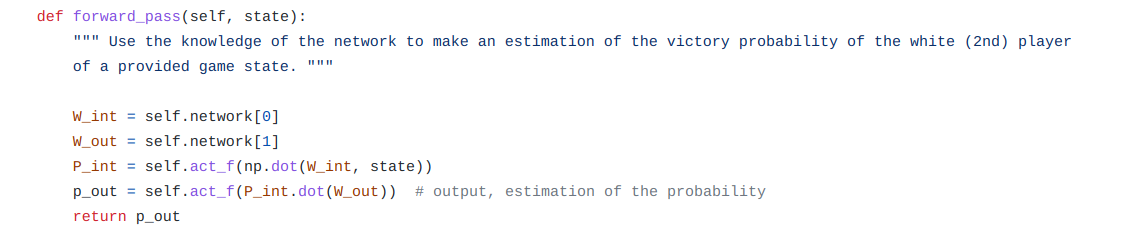
\includegraphics[width=\paperwidth]{forward_pass_code.png}}
      \caption{Implementation of the forward pass algorithm}
    \end{center}
\end{figure}

\subsubsection{Black and white player perspectives}

 To speed up the learning procedure and be able to use the same network to make predictions both as white and black, predictions will be considered as being from the point of view of white. Therefore, if the agent has to make a choice as black player, it will consider the complement of the probability estimations for the moves it can play. Indeed, taking the move with the smallest probability is in fact reducing the victory probability of the white player and therefore maximizing its.

\subsection{Learning strategies}

\subsubsection{Q-learning}

The first learning strategy used to train the neural network is Q-learning. At each turn, the difference ($\delta$) between the probability estimation of the actual state and the probability estimation of the most promising possible next state is computed. This value serves as the basis for the update of the network weights. The weights are updated with a \textit{backpropagation} algorithm. See the \hyperref[alg:backprop]{pseudocode} here, and the \hyperref[code:bp-code]{implementation} here.

\begin{algorithm}[H]
	\caption{Backpropagation for Q-learnign algorithm}
	\label{alg:backprop}
	\begin{algorithmic}[1]
	    \State $\delta \leftarrow p^{(out)}(s',W^{(int)},W^{(out)})-p^{(out)}(s*,W^{(int)},W^{(out)}) $
		\For {each neuron $i$ of intermediate layer}
		    \State $\Delta_{i}^{(int)} \leftarrow grad^{(out)} \cdot W_{i}^{(out)} \cdot grad_{i}^{(int)}$
    		\For {each neuron $j$ of input layer}
    		    \State $ W_{ij}^{(int)} \leftarrow W_{ij}^{(int)} - \alpha \cdot \delta \cdot \Delta_{i}^{(int)} \cdot X_{j} $
	    	\EndFor
	    	\State $ W_{i}^{(out)} \leftarrow W_{i}^{(out)} - \alpha \cdot \delta \cdot grad^{(out)} \cdot P_{i}^{(int)} $
	    \EndFor
	\end{algorithmic}
\end{algorithm}

\underline{Notations}: $s'$ is the current state, $grad$ is the derivative of the activation function and $s*$ is the state that the neural network evaluates as most promising for a given player.

\begin{figure}[H]
    \begin{center}
      \label{code:bp-code}
      \makebox[\textwidth]{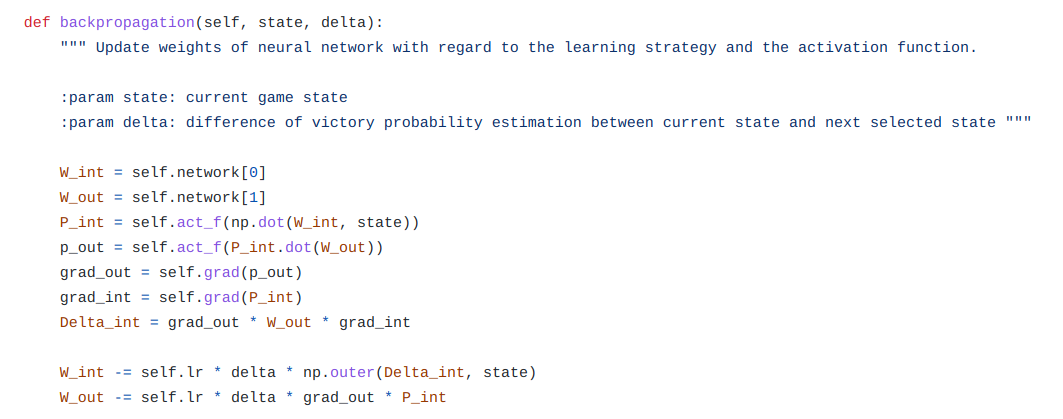
\includegraphics[width=\paperwidth]{backpropagation_code.png}}
      \caption{Implementation of the backpropagation algorithm}
    \end{center}
\end{figure}

\underline{Notations}: $self.grad$ refers to the derivative of the activation function.

\subsubsection{SARSA}

The SARSA learning rule is very similar to the Q-learning rule. The only difference is the state to which the current state is compared: in Q-learning, the comparison was made with the most promising state (independently of the choice made that turn) whereas in SARSA, the comparison is made with the state chosen at that turn.

\subsection{Activation functions}

Here are the different activation functions and their derivative considered in this project.

\begin{itemize}
    \item Sigmoïd
\end{itemize}

$$ \sigma(x) =  \frac{1}{1 + e^{-x}}  $$
$$ \sigma'(x) =  \sigma(x)(1 - \sigma(x))  $$

\begin{itemize}
    \item ReLU
\end{itemize}

$$ f(x) =  max(0, x)  $$
\[
    f'(x)=
\begin{cases}
    1,         & \text{if } x > 0\\
    0,         & \text{if } x < 0\\
    undefined & \text{if } x = 0
\end{cases}
\]

The value of the derivative is unedefined in $0$ as ReLU is non-differentiable in $0$. In this project, it will be arbitrarily set to 0 to avoid having to deal with undefined values and as this is the choice made by \href{https://hal.archives-ouvertes.fr/hal-03265059v2/document\#:~:text=The\%20value\%20of\%20the\%20derivative,the\%20subgradient\%20from\%20convex\%20analysis}{PyTorch and TensorFlow}.

\begin{itemize}
    \item Hyperbolic Tangent
\end{itemize}

$$ tanh(x) =  \frac{e^{x} - e^{-x}}{e^{x} + e^{-x}}  $$
$$ tanh'(x) = \frac{1}{cosh^{2}(x)}  $$

\subsection{Move selection rules}

\begin{itemize}
    \item Epsilon-greedy
\end{itemize}

The epsilon-greedy strategy depends on a parameter $\epsilon \in [0, 1]$. It will take the most promising move with a probability $1 - \epsilon$ and a random move (possibly the most promising) in other cases.

\begin{itemize}
    \item Softmax-exponential
\end{itemize}

The softmax-exponential strategy will always take a move randomly. The possible moves will be attributed a probability given by a softmax-exponential distribution and depending on their winning probability estimation. Let $S$ be the set of states that the agent can reach by mean of its available moves and $s$ one of these states having a probability estimation of $p_{s}$. This state will be attributed the probability: $\ddfrac{e^{p_{s}}}{\sum_{t \in S}{e^{p_{t}}}}$.


%%
%           MINIMAX AGENT
%%

\section{Minimax agent}
The MiniMax algorithm is Depth-First Search recursive algorithm. It can be seen as tree where each node is a state.
The root node is the current state and the child of a node is a state that can be reached after one move, from the parent state.
Considering that each player will the move in its higher interest, the algorithm imagine that the agent will play its best move, knowing that its opponent will always play its own best move (which is the worst move for the original agent).
%describe here the max and min logic

At each node is associated a value, which is the estimation of the value of the move. This estimation is necessary for the Minimax algorithm, it will be used by the agent to consider which move it will choose.

\begin{algorithm}[H] %%TODO ADD PRUNING !
	\caption{Minimax algorithm without prunning}
    \label{alg:minimax}
	\begin{algorithmic}[1]
	      \Function{minimax}{currentState, depth, player}
	      \If{$depth==0$ or gameOver()}
	            \Return evaluateState(state)
	       \EndIf
	       \If{$player == "MAX"$}
    	        \State $maxEval \gets -Infinity$
    	        \State $movesList \gets possibleMoves(sate, player)$
    	        \ForAll{m in movesList}
    	                \State $stateEval \gets $MINIMAX(m, depth-1, otherPlayer)
                        \State $maxEval \gets max(maxEval, stateEval)$
    	       \EndFor
    	       \State \Return maxEval

	       \Else
	            \State $minEval \gets Infinity$
    	        \State $movesList \gets possibleMoves(sate, player)$
    	       \ForAll{m in movesList}
    	       	     \State $stateEval \gets $ MINIMAX(m, depth-1, otherPlayer)
                     \State $minEval \gets max(minEval, stateEval)$
    	       \EndFor
    	       \State \Return minEval
	       \EndIf

	      \EndFunction

	\end{algorithmic}
\end{algorithm}
The efficiency of the algorithm depends on the \textit{Depth} parameter. This parameter is the depth of the tree, or, from a player perspective, the number of moves simulated in the future. With $Depth = 0$, the agent will play randomly (she doesn't simulate any move).
With $Depth = 1$, the agent will calculate the estimation for each possible move, but nothing more. With $Depth = 2$, the agent will also take into account the moves played by its opponent, etc.

The complexity of this algorithm is exponential : $0(b^m)$ where $b$ is the \textit{Depth} and $m$ is the number of possible move in each state.
It is obvious that the more futures moves are considered, the better will be the result, but also the more will be the computational power.

In order to optimize the algorithm, we implemented the pruning optimization. The idea is the following :
%--> describe the pruning

Our Minimax player has good result against human. The comparison of performance will be described in the Benchmark section\ref{sec:benchmark}.
Until depth = 3, the player select a move under the second.
For depth = 4 to 5, it may take a few seconds to choose a move, especially when the number of possible moves is high.
For depth = 6 and more, it takes at least 5 seconds, which is slow even for a human player.

\subsection{Heursitic}
As explained above, the algorithm assign a numerical value to a state, the \textit{estimation} or \textit{evaluation}. This evaluation is needed by the agent to estimate how much a move is interesting for him %him or it ?
or not. This evaluation is given by an heuristic, that is based on human strategies.
The heuristic return a value that depends on all these rules :
\begin{itemize}
    \item Which player won
    \item the number of corner owned by each player
    \item the number of pawns next to a corner
    \item empty squares next each player'pawns
    \item the number of pawn of each player
    \item the number of possible moves
\end{itemize}
The weight of each rule is a parameter that can be modified to improve the result. Obviously, the rules "the player win" and "the other player win", are weighted respectively
to \textit{infinity} and $-$\textit{infinity} (meaning that the agent will always select a move that will make hom move, and always avoid a move that will make him lose).
In order to improve the agent, we try different weigth. We can also compare two agents with the same algorithm and the same depth, but with different parameters.



-difficulté : easy for the strategy at the beginning, but difficult at the end, beaucause there are many things to thing about

 \newline
 After several test, we found those optimal weight for each heuristics:
\begin{itemize}
    \item Which player won : \textbf{1}
    \item the number of corner owned by each player : \textbf{1}
    \item the number of pawns next to a corner : \textbf{10}
    \item empty squares next each player'pawns : \textbf{2}
    \item the number of pawn of each player : \textbf{1}
    \item the number of possible moves : \textbf{3}
\end{itemize}


\section{Benchmark} \label{sec:benchmark}

\subsubsection{Test}
For the machine learning agent, we compared the different learning strategies combined with all the activation functions and different values for the rest of the parameters ( size of neural network, learning rate and random factors). We wanted to find the the optimal combinationof all those parameters to have the most competitive machine learning agent as possible.

Here is a list of the parameters we choose for comparaison:
\begin{itemize}
    \item Type of learning : \textit{ Q-learning, SARSA}
    \item Activation function: \textit{sigmoïd, ReLu, hyperbolic tangent}
    \item move selection: \textit{eps-greedy, softmax exponential}
    \item NN size: \textit{20, 40, 60, 80}
    \item learning rate: \textit{0.1, 0.2, 0.3}
    \item random factor: \textit{0.2, 0.3, 0.4}
\end{itemize}
We decided to compare one parameter at a time. It would have been better to try all combination of those parameters but it would have taken too much computation time. \\

We trained each agent for 7000 games and we compared each other for 200 games.
The value below are the percentage of win of the different paramaters. \\

\textbf{Learning strategies}
\newline
{\footnotesize (activation function: sigmoïd, move selection: eps-greedy, NN size: 40, learning rate: 0.2, random factor: 0.3)}
\newline
\begin{tabular}{|l|c|r|t|}
  \hline
  learning strategy (black) & Q-learning & SARSA & random\\
  \hline
  Q-learning & / & 53 & 87 \\
  SARSA & 44.5 & / & 87\\
  \hline
\end{tabular}
\newline

Q-learning performed a bit better than SARSA in this test. \\

\newline

\textbf{Activation function}
\newline
{\footnotesize(learning strategy: Q-learning, move selection: eps-greedy, NN size: 40, learning rate: 0.2, random factor: 0.3)}

\newline
\begin{tabular}{|l|c|r|t|v|}
  \hline
  activation function (black) & sigmoïd & ReLu & hyperbolic tangent & random \\
  \hline
  sigmoïd & / & 83 & 82 & 88.5\\
  ReLu & 11.5 & / & 43.5 & 45.5\\
  hyperbolic tangent & 29.5 & 67.5 & / & 73\\
  \hline
\end{tabular}
\newline

Sigmoïd activation function performed better than the 2 other on this test.

\newline

\textbf{move selection}
\newline
{\footnotesize(learning strategy: Q-learning, activation function: sigmoïd, NN size: 40, learning rate: 0.2, random factor: 0.3)}
\newline
\begin{tabular}{|l|c|r|t|}
  \hline
  move selection (black) & eps-greedy & softmax exponential & random\\
  \hline
  eps-greedy & / & 53 & 90.5\\
  softmax exponential & 37.5 & / & 89\\
  \hline
\end{tabular}
\newline

eps-greedy performed a bit better tha softmax exponential\\

\newline

\textbf{NN size}
\newline
{\footnotesize(learning strategy: Q-learning, activation function: sigmoïd, move selection: eps-greedy, learning rate: 0.2, random factor: 0.3)}
\newline

\begin{tabular}{|l|c|r|t|f|g|}
  \hline
  NN size (black) & 20 & 40 & 60 & 80 & random\\
  \hline
  20 & / & 42 & 49 & 41 & 90.5\\
  40 & 47.5 & / & 55 & 53 & 90.5 \\
  60  & 47 & 37 & / & 43 & 90\\
  80 & 54.5 & 42.5 & 54 & / & 88.5\\
  \hline
\end{tabular}
\newline

There is no obvious winner here, but NN size of 40 and 80 performed better than the other. As the NN size of 40 was better than the of 80 in their confrontetion, we decided to keep the value of 40 for the optimal NN size.

\newline

\textbf{learning rate}
\newline

{\footnotesize(learning strategy: Q-learning, activation function: sigmoïd, move selection: eps-greedy, NN size: 40, random factor: 0.3)}
\newline

\begin{tabular}{|l|c|r|t|g|}
  \hline
  learning rate (black) & 0.1 & 0.2 & 0.3 & random\\
  \hline
  0.1 & / & 47.5 & 42 & 91.5\\
  0.2 & 56.5 & / & 58.5 & 92\\
  0.3 & 56 & 42 & / & 91.5\\
  \hline
\end{tabular}
\newline

The best learning rate here is 0.2
\newline

\textbf{Random factor}
This random factor represent the epsilon in e-greddy algorithm
\newline

{\footnotesize(learning strategy: Q-learning, activation function: sigmoïd, move selection: eps-greedy, NN size: 40, learning rate: 0.2)}
\newline

\begin{tabular}{|l|c|r|t|g|}
  \hline
  random factor (black) & 0.2 & 0.3 & 0.4 & random\\
  \hline
  0.2 & / & 43.5 & 54 & 85.5\\
  0.3 & 52.5 & / & 56.5 & 85.5\\
  0.4 & 46 & 34.5 & / & 87\\
  \hline
\end{tabular}
\newline

The best random factor is 0.3

\newline

\subsubsection{Result}
With all those test, we conclude that the best combination of parameters was:
\begin{itemize}
    \item Type of learning : \textit{ Q-learning}
    \item Activation function: \textit{sigmoïd}
    \item move selection: \textit{eps-greedy}
    \item NN size: \textit{40}
    \item learning rate: \textit{0.2}
    \item random factor: \textit{0.3}
\end{itemize}

\subsubsection{comparison Minimax, ML}
We trained a ml agent with the parameters found in the previous chapter and trained for 7000 games with minimax with a depth of 3 for 100 games. Minimax won 58\% of the time

\section{Conclusion}

\end{document}